\chapter{Война}

\begin{figure}[H]
  \centering
  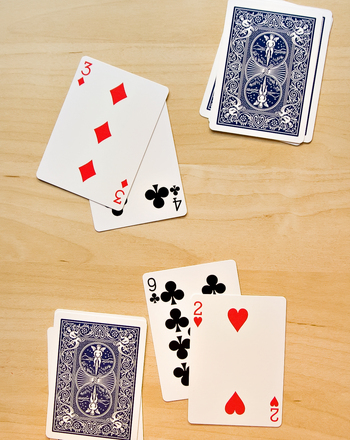
\includegraphics[width=1.0\linewidth,height=0.5\linewidth]{fig100001.png}
  \caption{„Война“ \\ https://images.squarespace-cdn.com/content/v1/59ea6080a803bb2f70ecbae5/1529350057743-92YH5Y0BN0JUMYB6X7NV/close-call-slide.jpg}
\label{fig100001}
\end{figure}

Играта „Война“ (Фиг. \ref{fig100001}) е детска игра с карти, като в основния си вариант се играе от двама играчи. Картите са стандартни, 52 карти за игра. Боите на картите са равноправни и няма сила по цвят. Всяка карта има сила с която участва в играта, като се започва от двойките (2 точки) и се стига до асата (14 точки). Тестето карти се разбърква и се раздава по равно на двамата играчи. Картите са с лицата на долу, като на всеки ход всеки от играчите показва най-горната карта. Играчът с по-силна карта взема и двете карти. Ако картите са с еднаква сила, то това е „война“ и играчите показват по три карти. Войната се печели от играча с по-силна трета карта. Ако и третите карти съвпадат, войната продължава, докато единият играч загуби войната. Спечелилият играч прибира всички карти, обърнати с лицето нагоре. Прибраните карти винаги застават най-отдолу в тестето на съответния играч. Играта се губи от този играч, който остане без карти. 

Играта е относително проста и не изисква специални умения, което я прави идеален вариант за малки деца. Работата по изработването на тази игра, под формата на мобилно приложение, започва със създаването на нов проект (Фиг. \ref{fig100002}).

\begin{figure}[H]
  \centering
  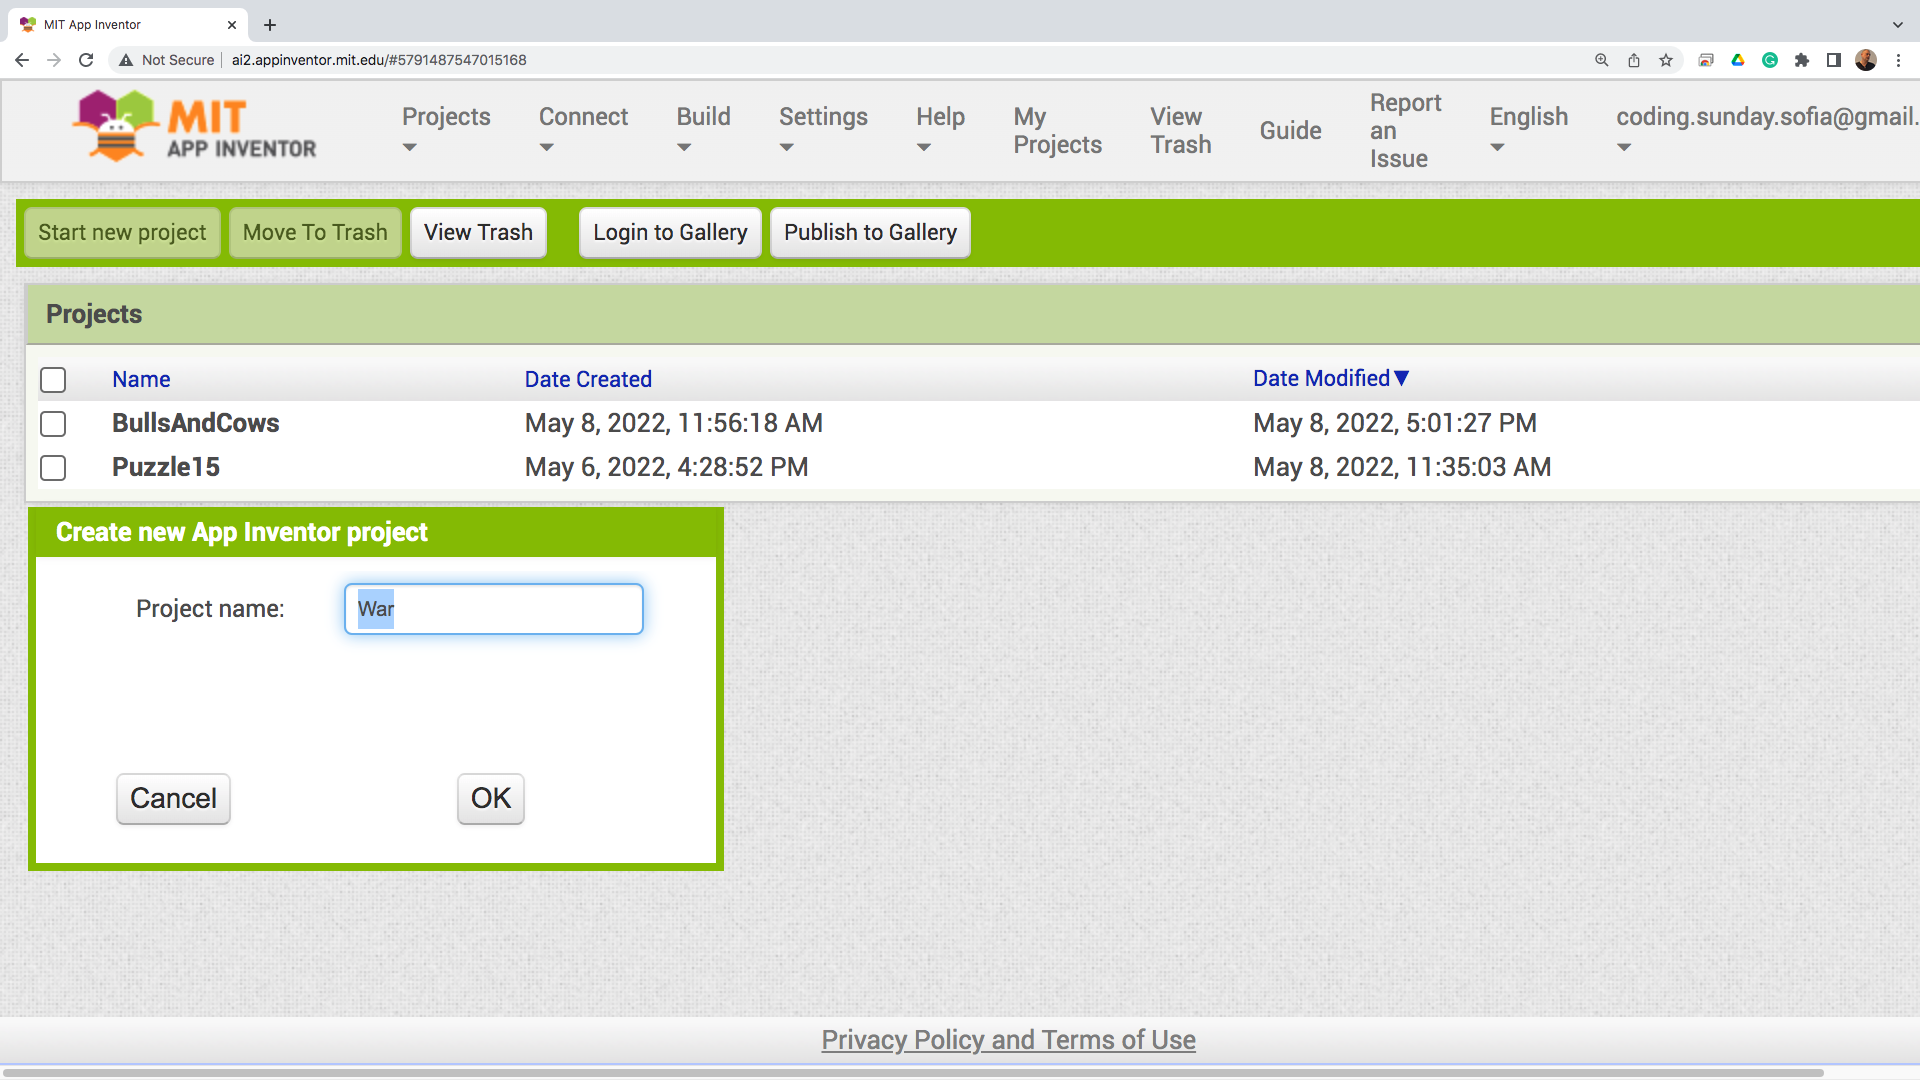
\includegraphics[width=1.0\linewidth,height=0.5\linewidth]{fig100002.png}
  \caption{Създаване на нов проект за играта „Война“}
\label{fig100002}
\end{figure}

Потребителският интерфейс ще бъде възможно най-опростен. Два бутона (Фиг. \ref{fig100003}), най-отгоре в работното пространство, ще служат за стартиране на нова игра и направата на ход.

\begin{figure}[H]
  \centering
  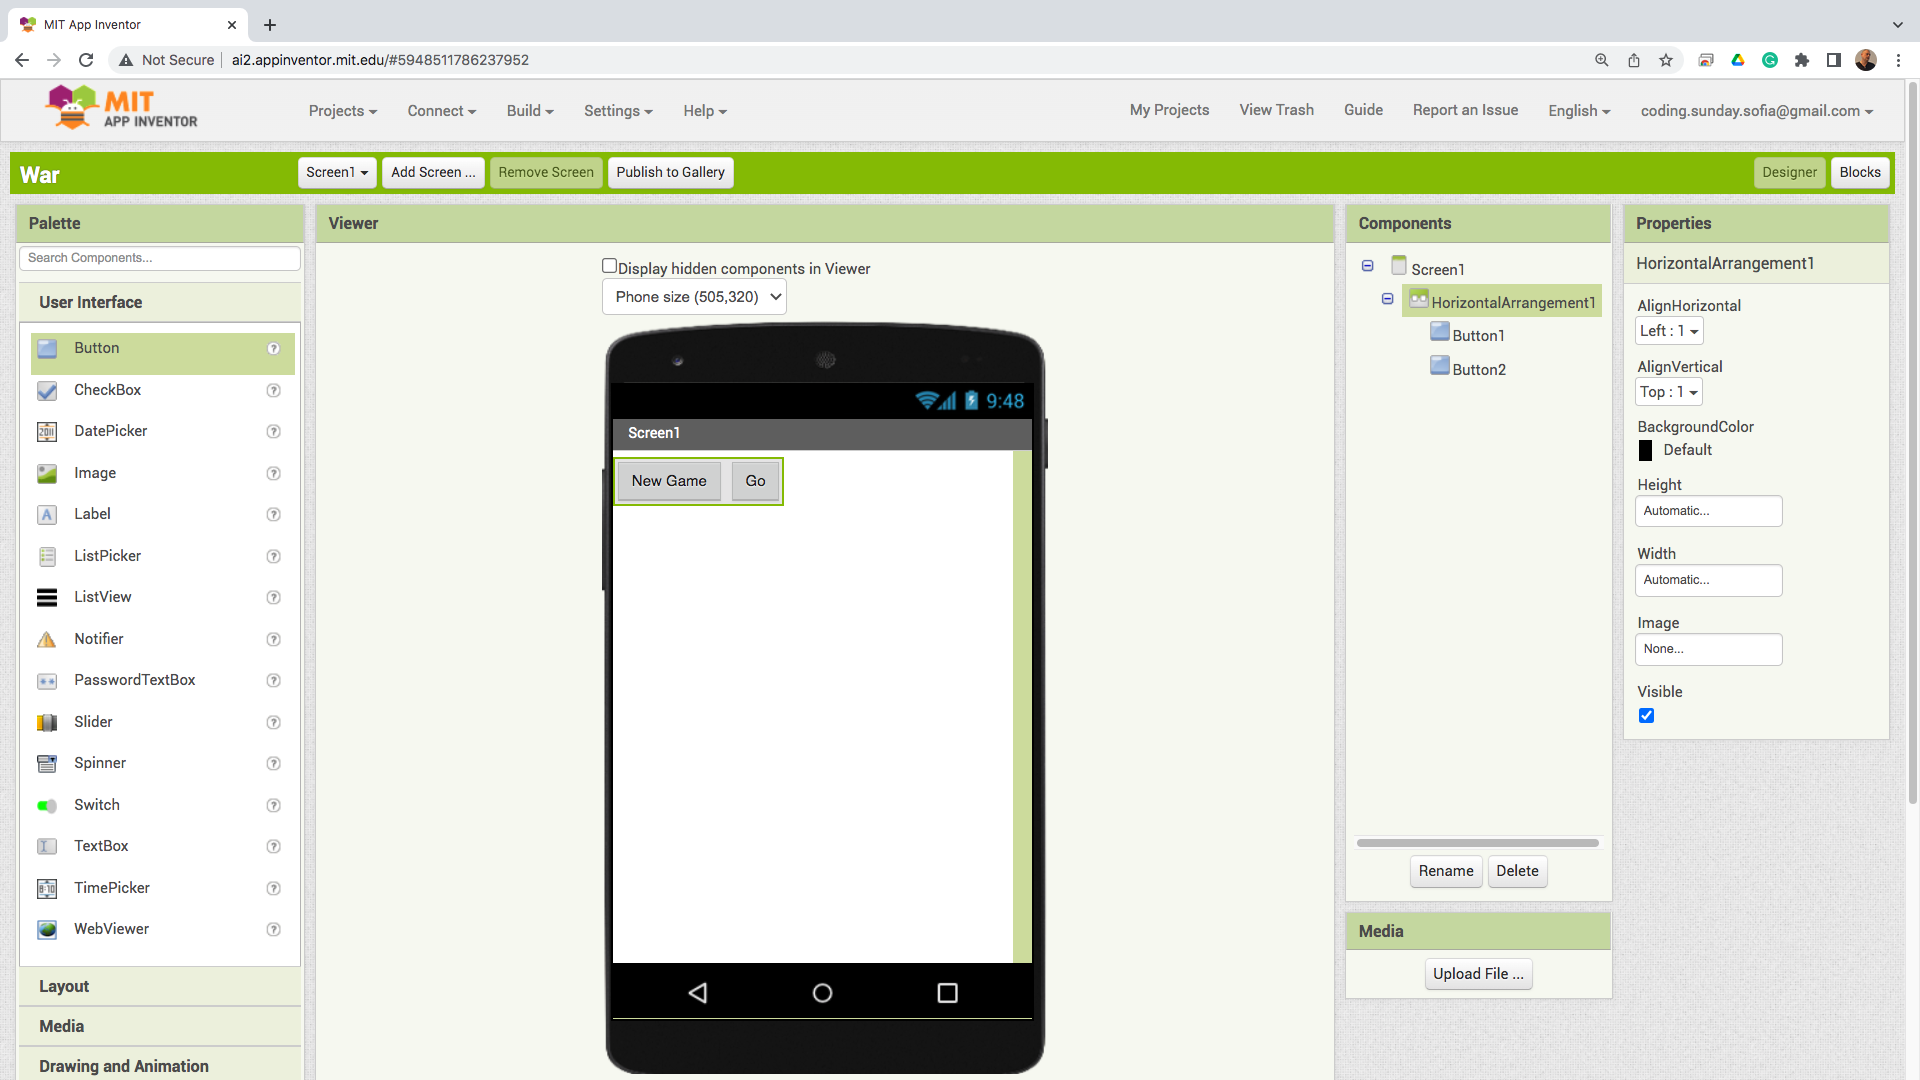
\includegraphics[width=1.0\linewidth,height=0.5\linewidth]{fig100003.png}
  \caption{Бутони за стартиране на нова игра и направа на ход}
\label{fig100003}
\end{figure}

Веднага под бутоните, в табличен вид се подреждат два реда с визуални компоненти за показване на графични изображения (Фиг. \ref{fig100004}). В първата колона ще се визуализира гръб на карта, което символизира тестетата на двамата играчи, а в другите три съседни компонента ще се показва една карта, когато няма война и три карти, когато има война. 

\begin{figure}[H]
  \centering
  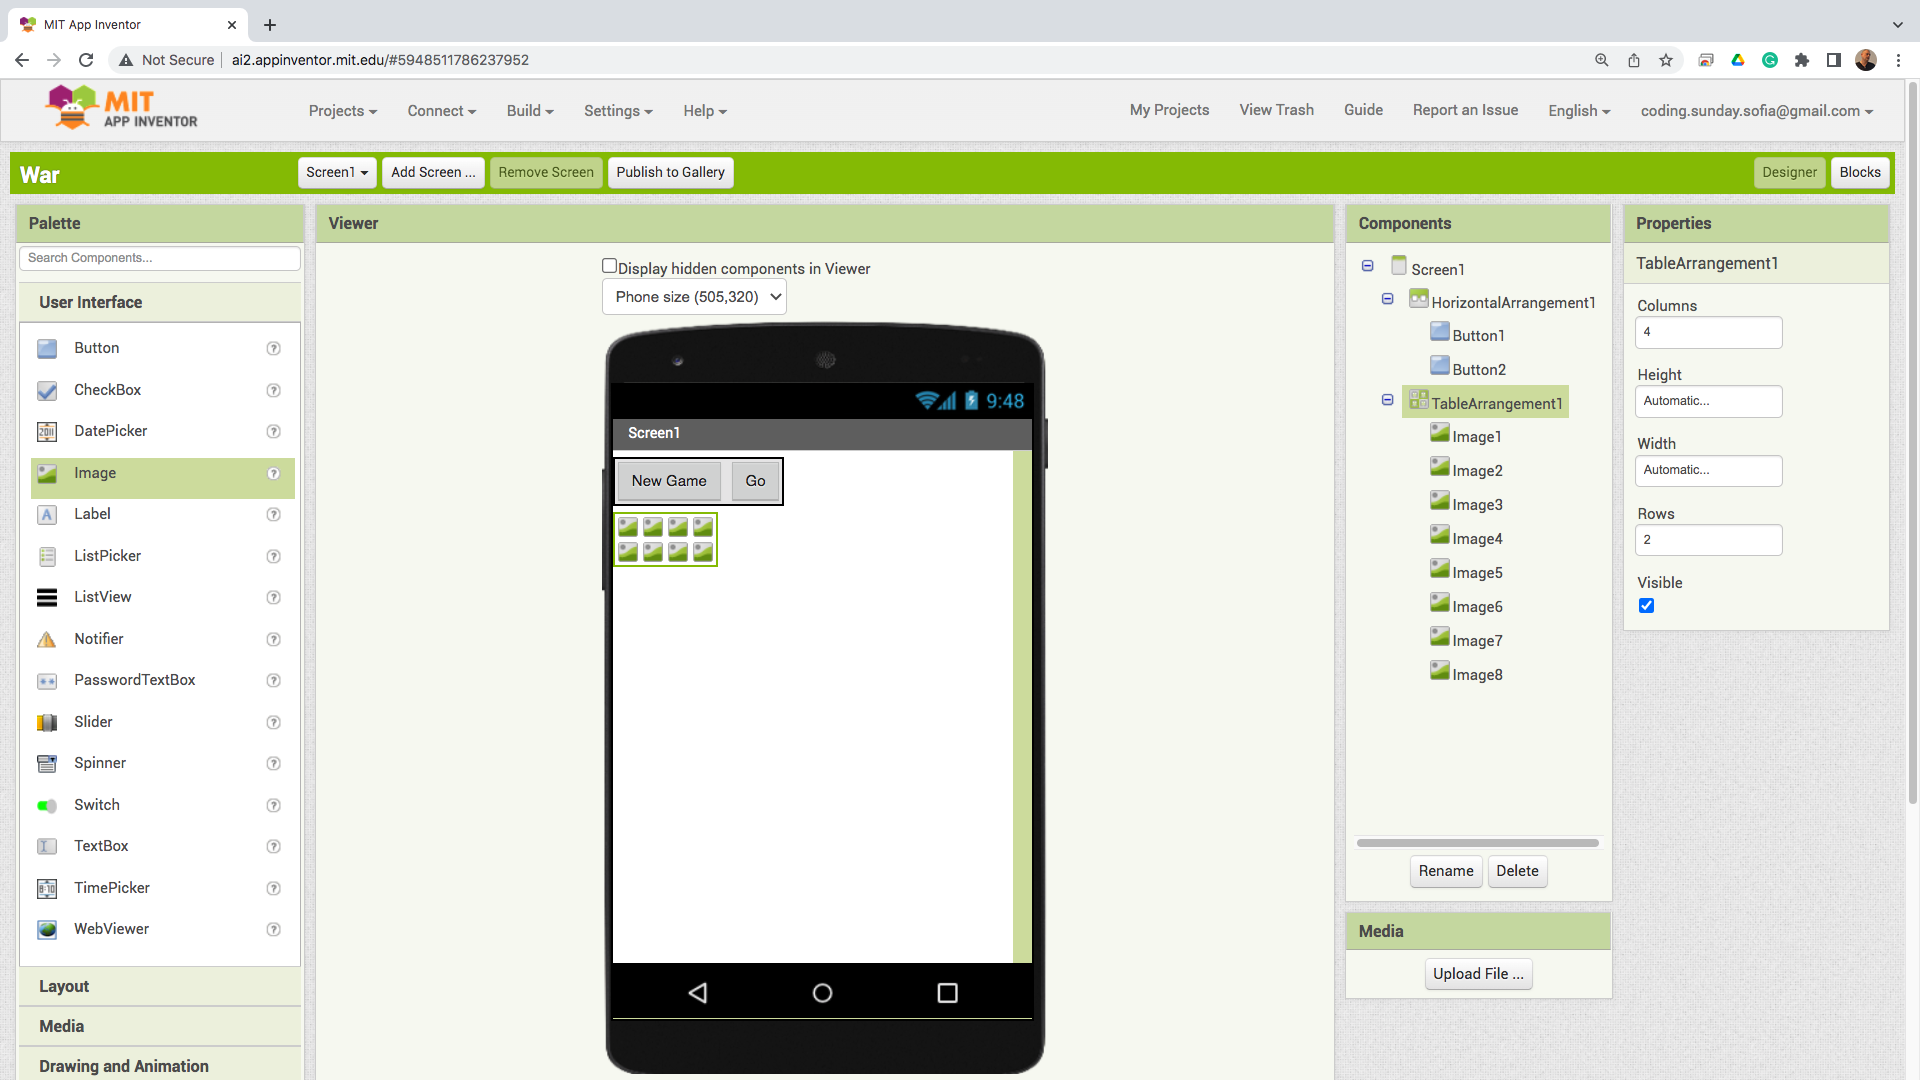
\includegraphics[width=1.0\linewidth,height=0.5\linewidth]{fig100004.png}
  \caption{Компоненти за визуализация на картите}
\label{fig100004}
\end{figure}

За изображенията на самите карти може да се използва всеки комплект от карти, които се разпространяват със свободен лиценз за не търговска употреба (Фиг. \ref{fig100005}).

\begin{figure}[H]
  \centering
  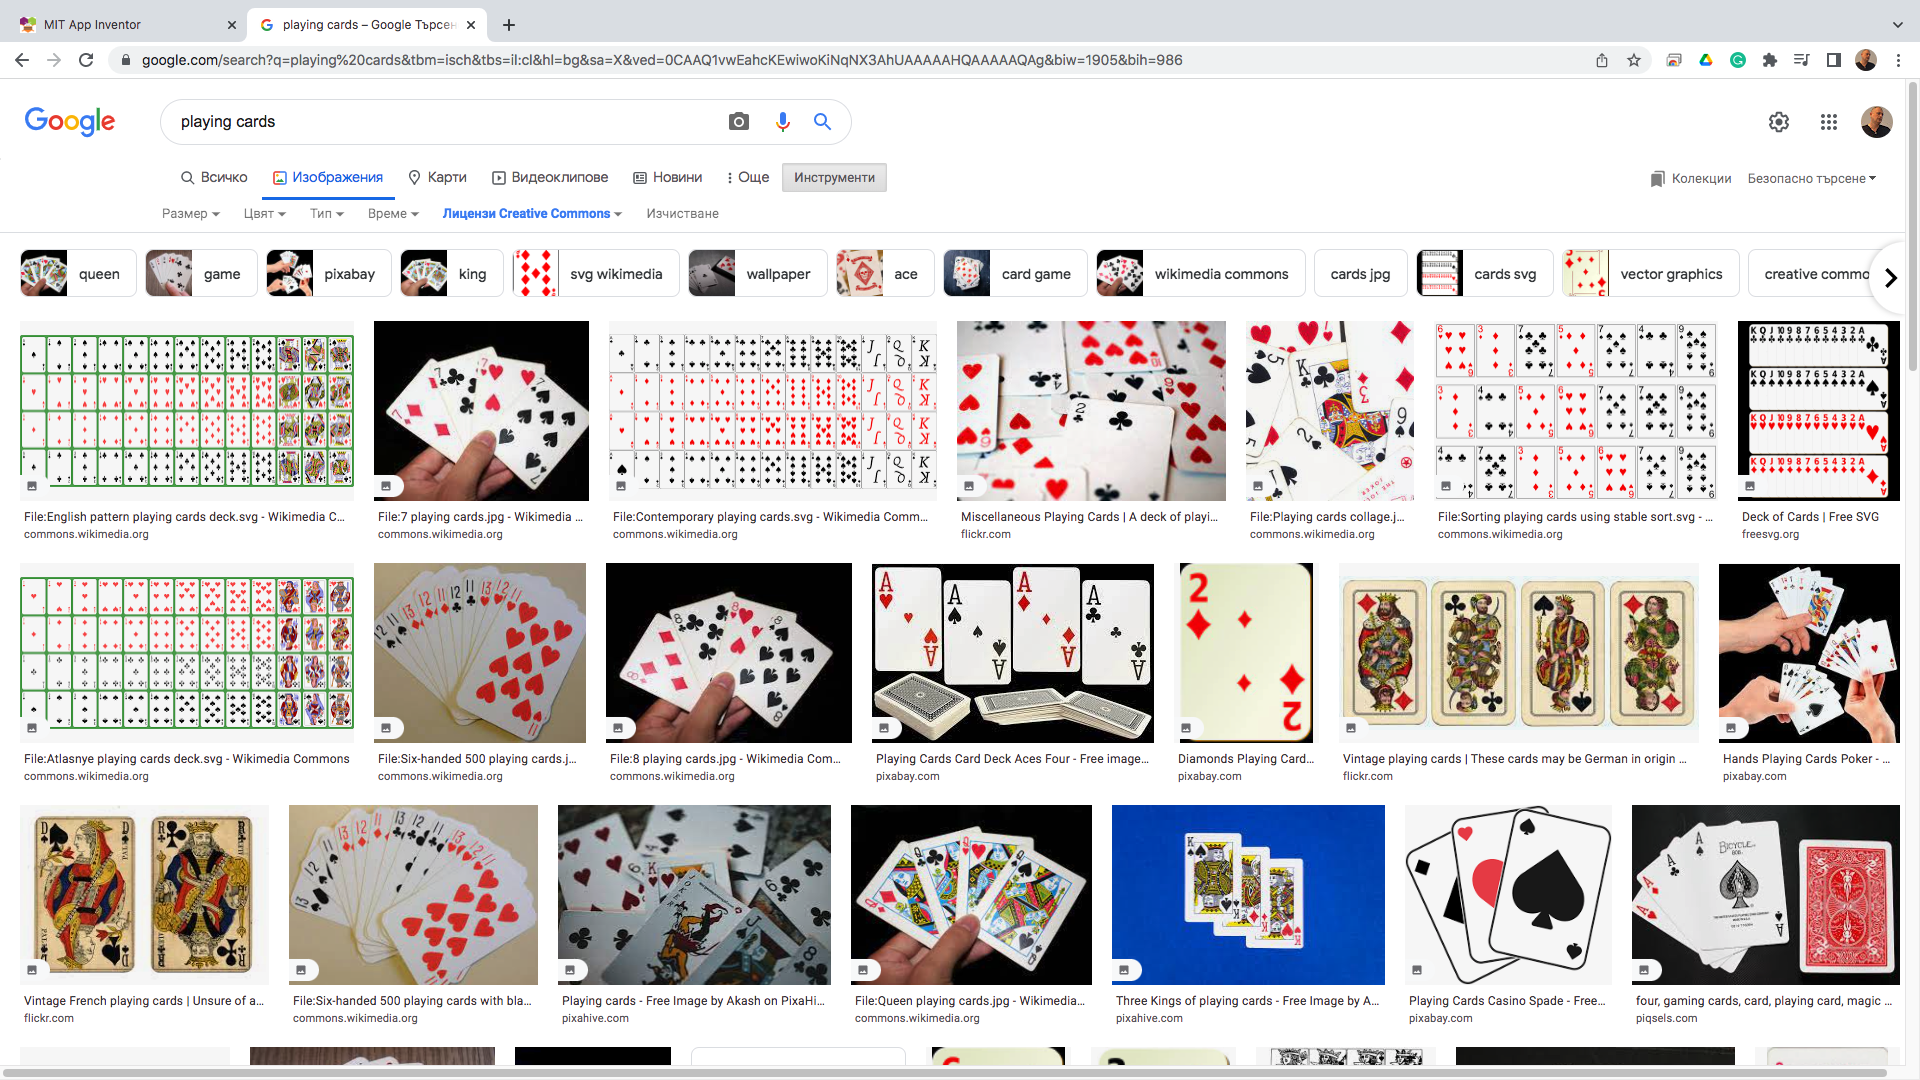
\includegraphics[width=1.0\linewidth,height=0.5\linewidth]{fig100005.png}
  \caption{Изображения на карти за игра}
\label{fig100005}
\end{figure}

Ако комплектът карти е в общо изображение, то се нарязва на 52 отделни изображения и поне едно изображение за гръб на картите. Така подготвените 53 графични файла, се зареждат в проекта, като се качват файл по файл (Фиг. \ref{fig100006}).

\begin{figure}[H]
  \centering
  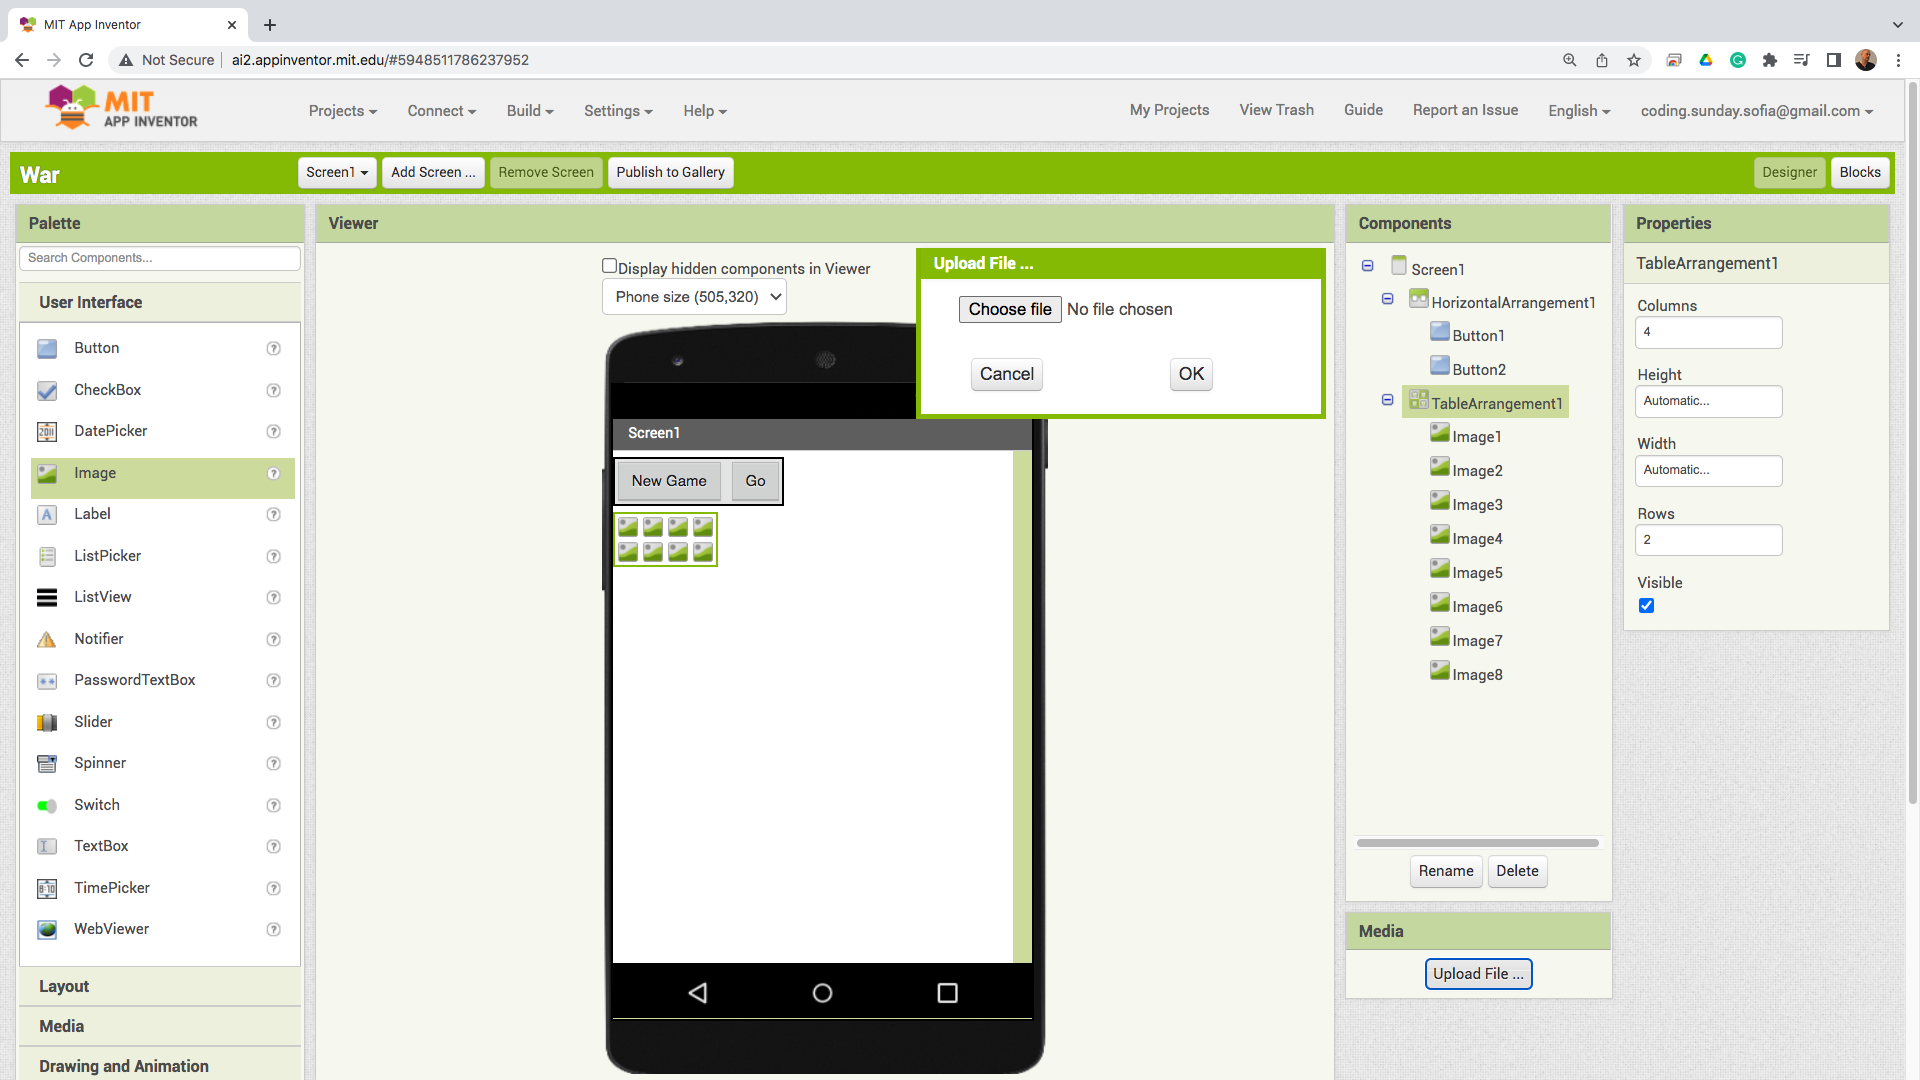
\includegraphics[width=1.0\linewidth,height=0.5\linewidth]{fig100006.png}
  \caption{Качване на графични файлове}
\label{fig100006}
\end{figure}

От така качените графични файлове, в първата колона от изображения се зарежда изображението за гръб на картите (Фиг. \ref{fig100007}).

\begin{figure}[H]
  \centering
  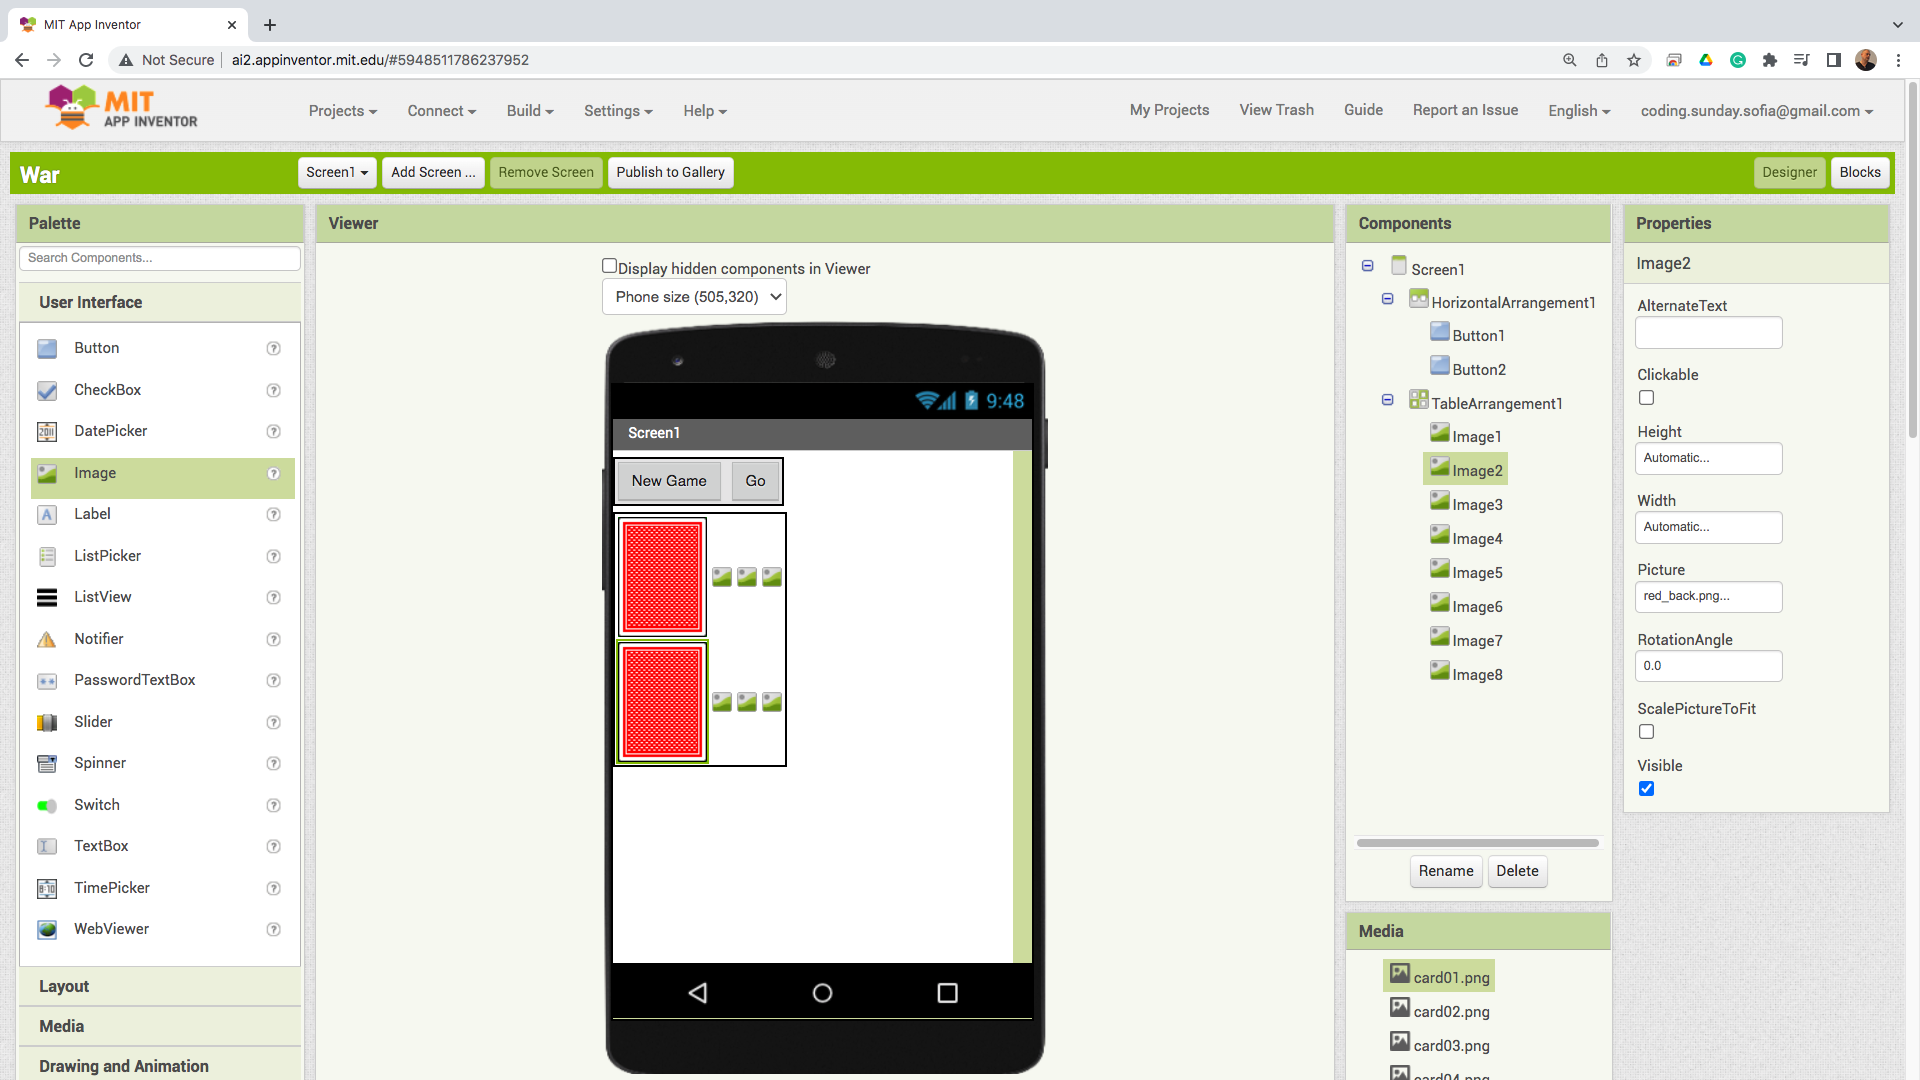
\includegraphics[width=1.0\linewidth,height=0.5\linewidth]{fig100007.png}
  \caption{Изображения за маркирането на тестетата}
\label{fig100007}
\end{figure}

Картите ще циркулират в модела на играта под формата на цели числа. За тази цел се обявяват пет помощни, глобални променливи - списък с основното тесте, два списъка за картите държани от играча и два списъка за картите поставени на масата от играчите (Фиг. \ref{fig100008}). 

\begin{figure}[H]
  \centering
  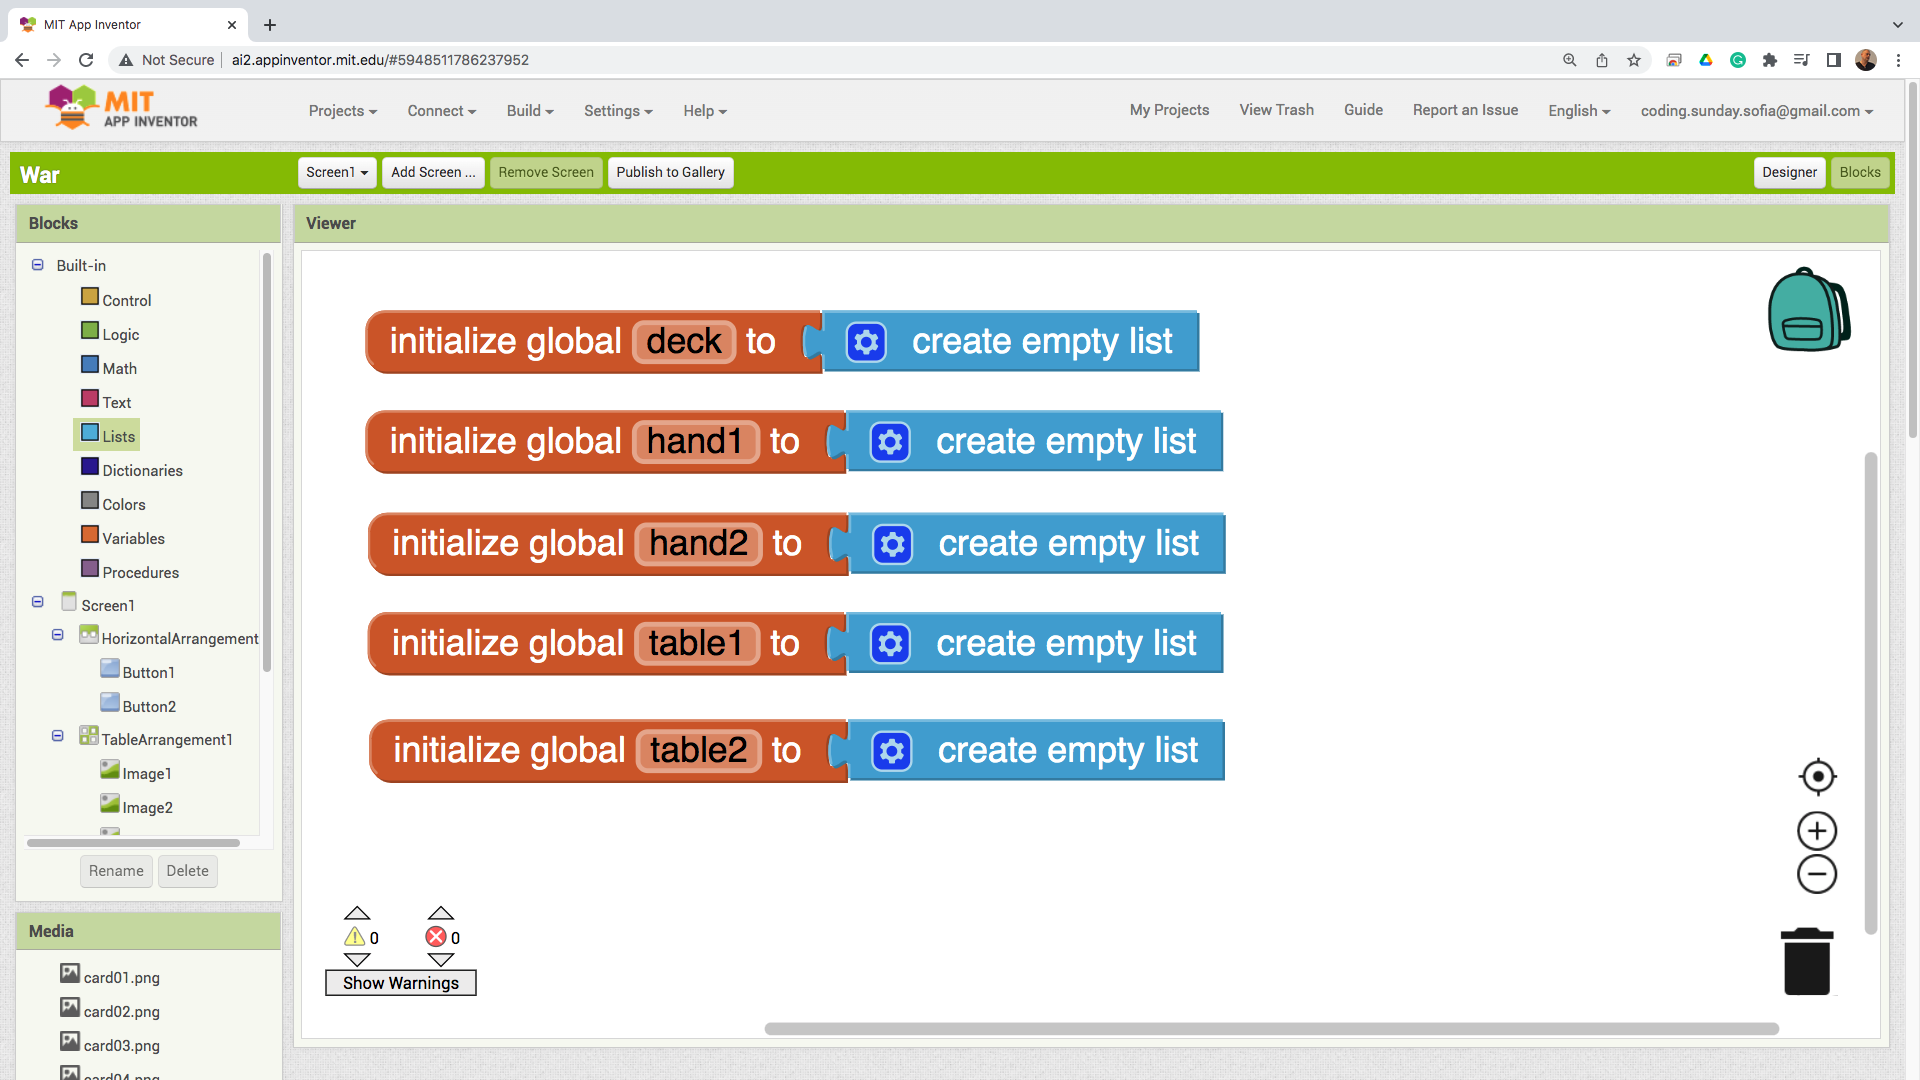
\includegraphics[width=1.0\linewidth,height=0.5\linewidth]{fig100008.png}
  \caption{Основни помощни променливи}
\label{fig100008}
\end{figure}

Два допълнителни списъка биха улеснили визуализацията на картите, които се поставят на масата. В тези списъци се поместват отпратки към визуалните компоненти за показване на изображения (Фиг. \ref{fig100009}).

\begin{figure}[H]
  \centering
  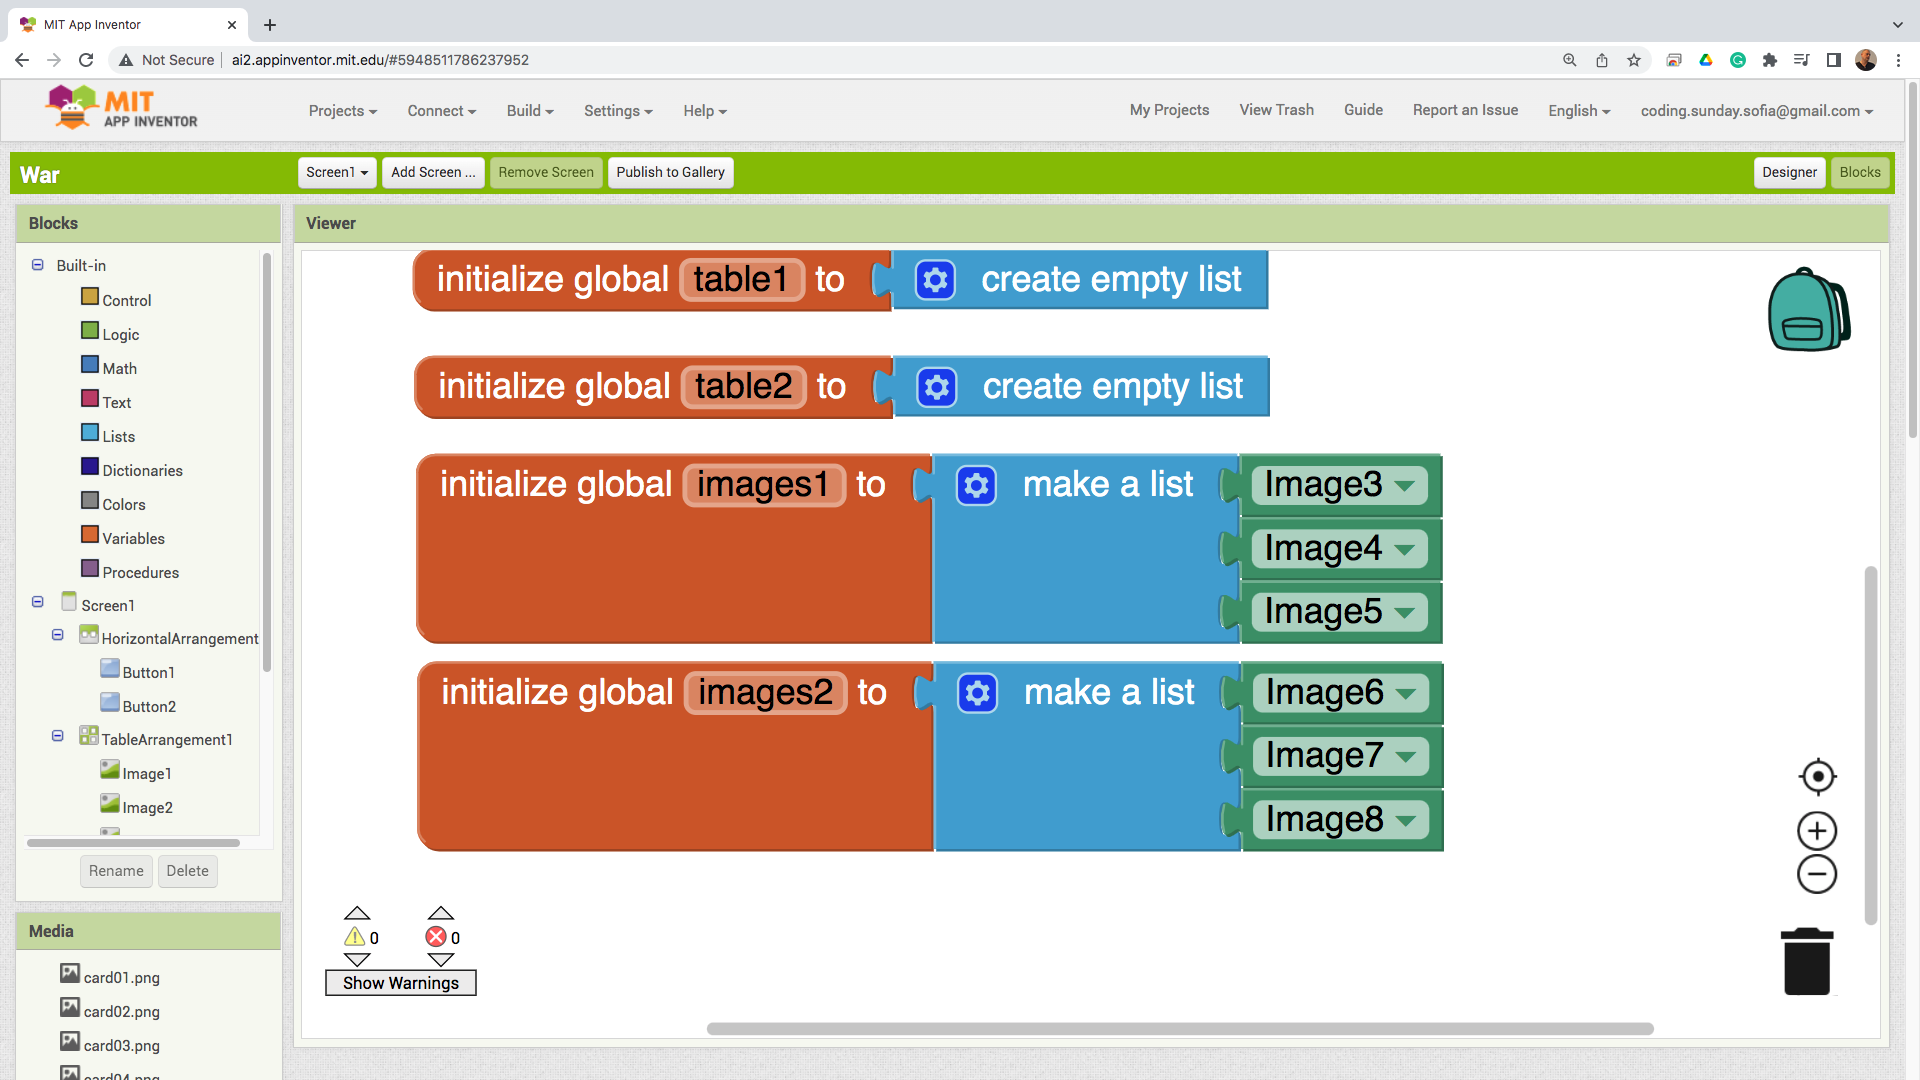
\includegraphics[width=1.0\linewidth,height=0.5\linewidth]{fig100009.png}
  \caption{Помощни списъци за визуализация}
\label{fig100009}
\end{figure}

Последната помощна променлива подрежа в списък изображенията на картите. Подредбата е важна, като двойките стоят на първите четири места, на вторите четири места стоят тройките и така нататък, докато се стигне до последните четири места на които стоят асата (Фиг. \ref{fig100010}). Благодарение на тази подредба, при пресмятането на победителите в отделните рундове ще се постига с просто аритметично пресмятане. 

\begin{figure}[H]
  \centering
  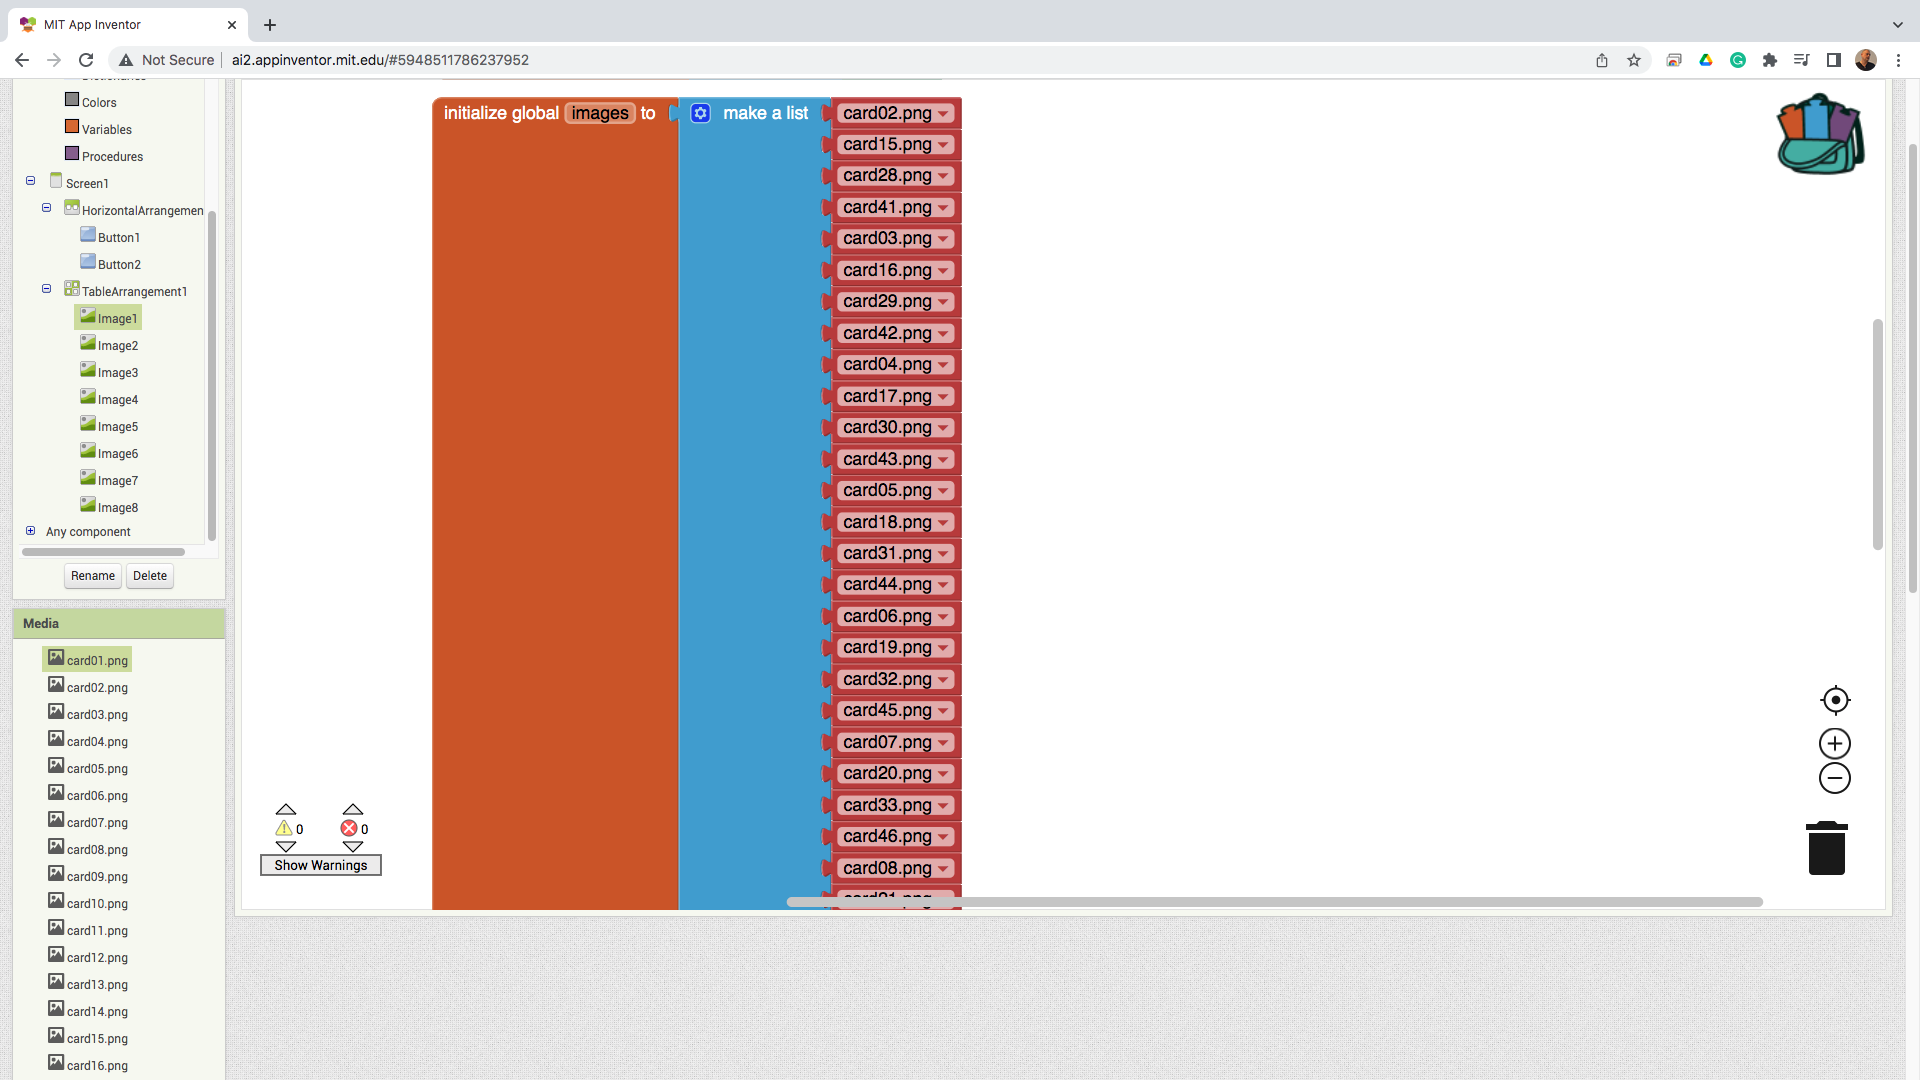
\includegraphics[width=1.0\linewidth,height=0.5\linewidth]{fig100010.png}
  \caption{Помощна променлива за реда на картите по сила}
\label{fig100010}
\end{figure}

